
\chapter{Ultra-peripheral Collisions at the Large Hadron Collider}

\section{Ultra-peripheral Heavy-Ion Collisions}

Similar to the Rutherford experiment, in heavy-ion collisions the scattered particles carry information about the internal structure of the nucleus. 

The Rutherford experiment has the three components that still characterize high-energy nuclear experiments: a probe, a medium, and a signal. Alpha particles probe the medium of the gold atom, and the angular distribution of scattered alpha particles signals the internal structure of the atom. 

Ultra-peripheral collisions occur at impact parameters greater than the sum of the heavy-ion radii. In these collisions, hadronic interactions are strongly suppressed while photonuclear activity is enhanced proportional to the square of the nuclear charge. The electromagnetic field of an incoming heavy-ion, from the perspective of a target, is equivalent to a flux of virtual photons; figure \ref{fig:smushedField} illustrates the Lorentz contraction of the field of a boosted charge.

\begin{figure}[h!]
\begin{centering}
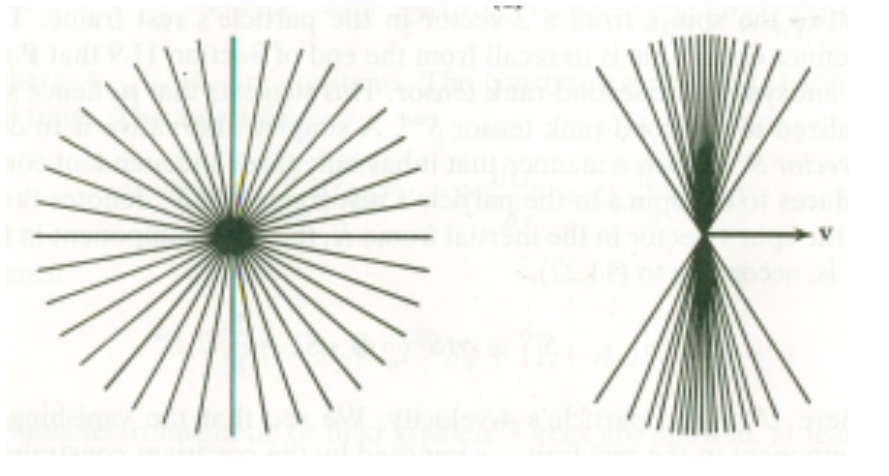
\includegraphics[width=4in]{Chapter1/importfigs/jackson_em_wwa.png}
\par\end{centering}
\caption{ (a.) electromagnetic field of stationary charge (b.) eletromagnetic field of boosted charge \cite{WWJackson}. \label{fig:smushedField}}
\end{figure}

The Weizsacker-Williams appoximation (WWA) calculates the density of photons, about the nucleus, as a function of energy. WWA is a semi-classical formulation. Maxwell's equations are solved for a stationary point charge boosted to an ultra-relativistic velocity. In the target's frame, the Fourier transform of the source field is taken. The Fourier frequency modes are interpreted through the quantum mechanical equation of photon energy. The photon flux as function of energy is given by
\begin{equation}
N(\omega,b) = \frac{\alpha}{\hbar \omega}\left( \frac{Z}{b\beta\pi} \right)^2\left ( \frac{\omega b}{\gamma \nu} \right )K_1^2\left ( \frac{\omega b}{\gamma \nu} \right ) ,
\end{equation}
where $\alpha$ is the QED coupling constant, $\omega$ is the photon energy, $Z$ is the atomic number of the nuclei, $b$ is the impact parameter, $\beta$ is ratio of the nuclei speed to the speed of light, $\gamma$ is the Lorentz boost of the nuclei, $K_1^2$ is a Bessel function, $\nu$ is the photon frequency \cite{WWJackson}.

Gluons are the particle exchanged in strong interactions. However, gluons themselves carry color charge. By analogy, photons transmit the electromagnetic force, but do not themselves have an electric charge. The gluons are spin-1, meaning that more than one can occupy the same quantum state.

When a quark is scattered from a nucleus, the strong force field lines for a tube between the quark and its counterpart. Given that the strong coupling constant increases with distance the strong interaction gathers potential energy until the threshold for quark production is passed, at which point an anti-quark is generated to screen the ejected quark. These quarks continue to separate from each other and continue the quark generation process. The resulting final state hadron distribution takes the form of a cone centered on the path of the initial quark. 

QCD factorisation describes the diffractive-photoproduction dijet cross-section as the convolution of the partonic cross-section with the diffractive parton distributions. However, factorisation only describes H1 data if the resolved-photon contribution is suppressed. 

The photoproduction cross-section is proportional to the gluon distribution. At low momentum transfer, photons interact electromagnetically, i.e. directly, with partons. High energy, "resolved" photons possess a hadronic structure; instead of directly interacting with the nuclei, these photons fluctuate into mediating quark-antiquark pairs. 

\section{Vector Meson Photoproduction}

The virtual photons present in UPC can fluctuate into a quark-antiquark pair which can take the form of a low mass meson. This meson then interacts with the target nuclei via colorless gluon exchange, emitting a vector meson. If the virtual photon interacts coherently with the target nucleus, this is reflected in the transverse momentum of the vector meson. The vector meson decays into a dilepton pair detectable by CMS. 

Ultra-peripheral coherent $J/\Psi$ photoproduction was studied in the ALICE 2011 Pb-Pb data. 

\begin{figure}[h!]
\begin{centering}
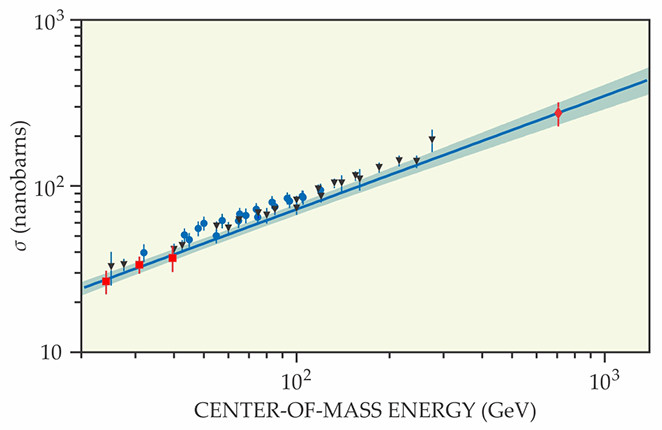
\includegraphics[width=4in]{Chapter2/importfigs/aliceData1.jpeg}
\par\end{centering}
\caption{$\gamma +$proton$\rightarrow J/\Psi +$proton cross-section. \label{fig:aliceData1}}
\end{figure}

CMS has studied $J/\Psi$ and $\rho$ photoproduction off the proton in proton-Pb collisions. 

\begin{figure}[h!]
\begin{centering}
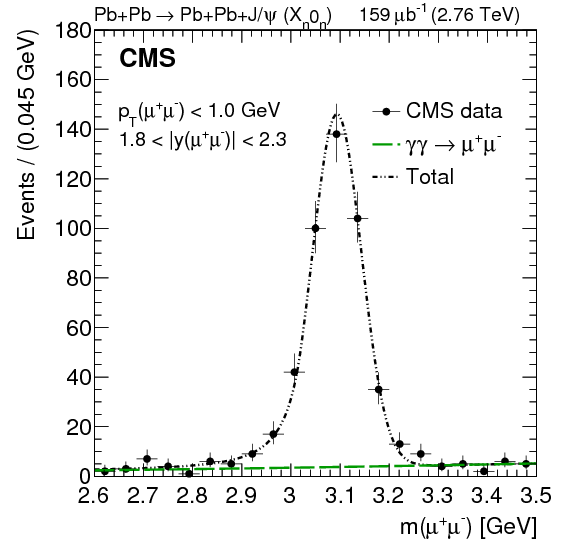
\includegraphics[width=4in]{Chapter2/importfigs/patkenny_Figure_001-a.png}
\par\end{centering}
\caption{Pat Kenny Plot 1 \label{fig:pk3}}
\end{figure}


\begin{figure}[h!]
\begin{centering}
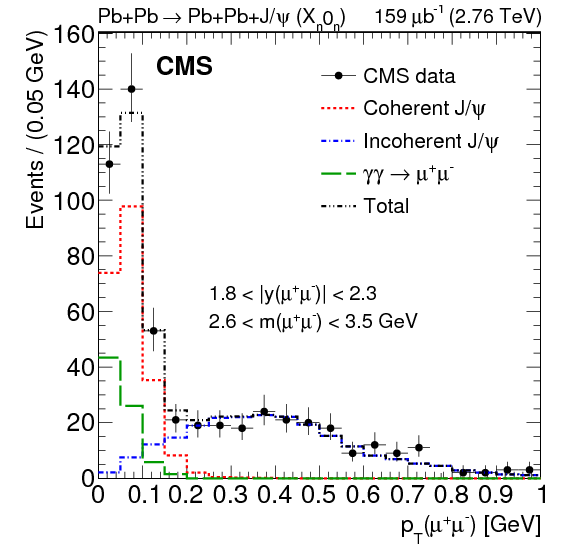
\includegraphics[width=4in]{Chapter2/importfigs/patkenny_Figure_001-b.png}
\par\end{centering}
\caption{Pat Kenny Plot 2 \label{fig:pk2}}
\end{figure}

\begin{figure}[h!]
\begin{centering}
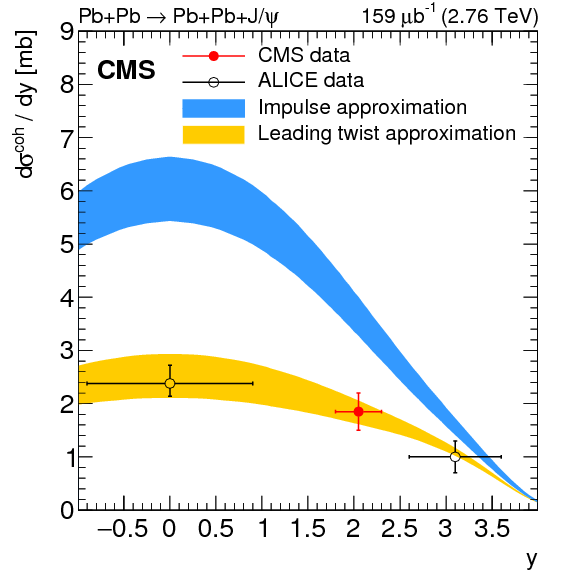
\includegraphics[width=4in]{Chapter2/importfigs/patkenny_Figure_002.png}
\par\end{centering}
\caption{Pat Kenny Plot 3 \label{fig:pk3}}
\end{figure}


\section{Photon-Photon Interactions}

Classical electrodynamics forbids the scattering of a photon off another photon.

The polarization of the vacuum is a consequence of quantum mechanics. Around a photon there is a cloud of particle-antiparticle pairs, appearing together and then annihilating each other after a time proportional to their energy. In so far as these particles have an electric charge, portions of the local area may carry a non-zero electric charge. Thus, two photons may scatter off each other in three possible exchanges: Diagrams for Delbrück scattering, photon splitting, and elastic light-by-light scattering. 

\begin{figure}[h!]
\begin{centering}
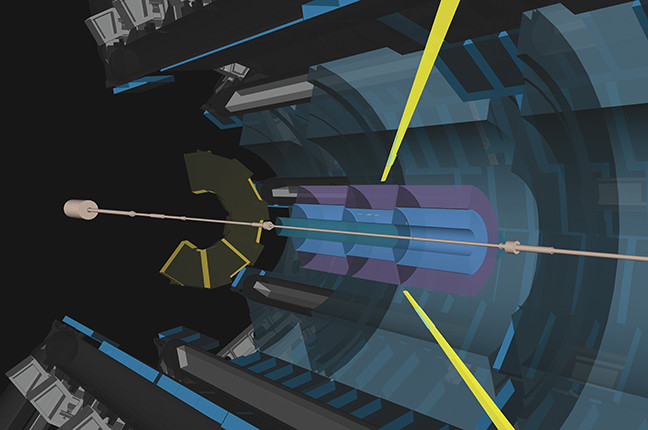
\includegraphics[width=4in]{Chapter2/importfigs/gammaGammaAtlasEvent.jpeg}
\par\end{centering}
\caption{Event Display of ATLAS photon-photon scattering \label{fig:atlasEvent}}
\end{figure}

\section{Dijet Photoproduction}

The dijet photoproduction cross-section, like that of vector meson photoproduction, displays diffractive dips in its $|t|$ dependence. Furthermore, according to the color glass condensate formalism, coherent dijet production is sensitive to gluon saturation effects at small Bjorken-x values. Gluon saturation would affect the color-dipole orientation of nucleons in the transverse plane. This effect should be reflected in an enhanced azimuthal angle correlation of the jets. 

\subsection{Factorization}

Diffractive dijet photoproduction is not describable in perturbative QCD. For coherent processes the photon energy is small, and therefore the wavelength is large compared to the size of the nucleus. At these large distances, there isn't a hard scale, and so perturbation calculations cannot be done. Gluon splitting interactions dominate the low Bjorken-x partons. QCD collinear factorization describes these soft interactions via the convolution of parton cross sections, taken from perturbative QCD, and diffractive parton distribution functions, taken from experiment \cite{Andreev:2015cwa}. 

\begin{figure}[h!]
\begin{centering}
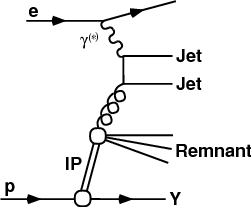
\includegraphics[width=2.2in]{Chapter1/importfigs/fig1a.png}
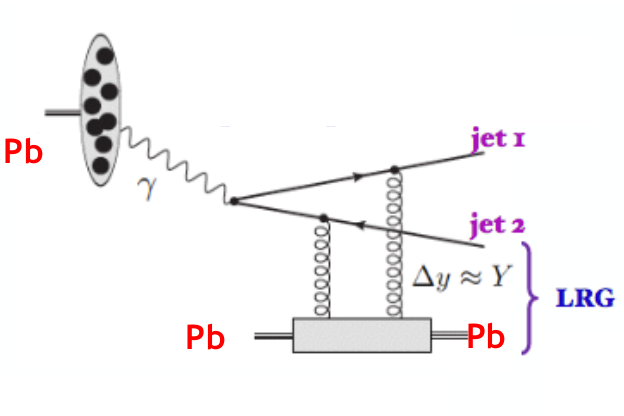
\includegraphics[width=3in]{Chapter1/importfigs/fig3_daniel_upc.png}
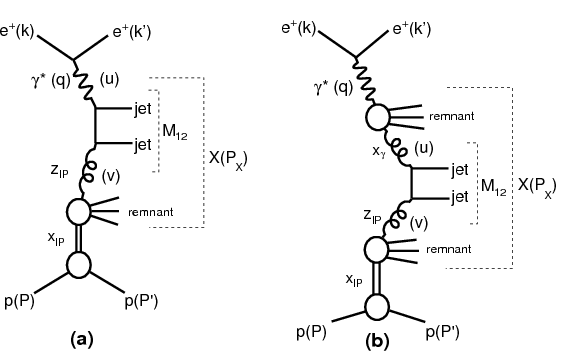
\includegraphics[width=6in]{Chapter1/importfigs/h1_2015_feyn.png}
\par\end{centering}
\caption{Feynman diagrams for coherent jet photoproduction in (upper a.) lepton-proton collisions, (upper b.) Pb-Pb collisions, (lower a.) direct-photon in ep, (lower b.) resolved-photon in ep. \label{fig:feynmanUPC1}}
\end{figure}

In electron-hadron collisions, diffractive photoproduction is characterized by the presence of a large rapidity gap in the final state and an intact nucleus. The Feynman diagram of electroproduction in lepton-hadron collisions is similar to that of photoproduction in ultraperipheral collisions, as seen in fig.\ref{fig:feynmanUPC1}. The diffractive dijet cross section is expressed by the convolution of partonic cross sections $d\hat{\sigma}$ and diffractive PDFs $f^D_{i/p}$.
\begin{equation}
d\sigma (ep \rightarrow e + 2 jets + X^{'} + p) = \sum_{i} \int dt \int dx_\mathbb{P} \int dz_\mathbb{P}d\hat{\sigma}_{ei\rightarrow 2jets}(\hat{s},\mu^2_R,\mu^2_F)\times f^D_{i/p}(z_\mathbb{P},\mu^2_F,x_\mathbb{P},t) ,
\end{equation}
where $x_\mathbb{P}$ is longitudinal momenetum fraction lost by the incoming proton, $d\hat{\sigma}_{ei\rightarrow 2jets}$ is the partonic cross-section for the process, $z_\mathbb{P}$ is the longitudinal momentum fraction of the pomeron entering the hard process, $\hat{s}$ is the squared invariant energy of the subprocess, $\mu^2_R$ is the squared renormanlization scale, $\mu^2_F$ is the squared factorisation scale, $f^D_{i/p}$ is the diffractive parton distribution,and $t$ is the four-momentum transfer squared at the vertex. 

In the proton-vertex factorisation hypothesis, the dependence on $x_{\mathbb{P}}$ and $|t|$ is factored out of the dependence on $\mu^2_F$ and $z_{\mathbb{P}}$. Furthermore, $f^D_{i/p}$ is sum of contributions from the pomeron and Reggeon:
\begin{equation}
f^D_{i/p}(z_{\mathbb{P}},\mu^2_F,x_{\mathbb{P}},t) = f_{\mathbb{P}/p}(x_{\mathbb{P}},t)f_{i/\mathbb{P}}(z_{\mathbb{P}},\mu^2_F) + n_\mathbb{R}f_{\mathbb{R}/p}(x_{\mathbb{P}},t)f_{i/\mathbb{R}}(z_{\mathbb{P}},
\mu^2_F) ,
\end{equation}
where $_{\mathbb{P}/p}$ is the pomeron flux factor, $f_{\mathbb{R}/p}$ is the Reggeon flux factor, $n_\mathbb{R}$ is the normalization factor of the Reggeon, $f_{i/\mathbb{P}}$ is the pomeron parton distribution, and $f_{i/\mathbb{R}}$ is the Reggeon parton distribution.

Lepton-hadron collisions were performed at HERA and measured by the H1 experiment. These experiments reported a value for the total diffractive photoproduction cross section that is double that predicted by QCD collinear factorization; fig.\ref{fig:h1Ratio} compares the cross-section of H1 data to that predicted by NLO-QCD. Diffractive events were selected for using rapidity gaps or the presence of leading protons in the very forward proton spectrometer (VFPS). 

\begin{figure}[h!]
\begin{centering}
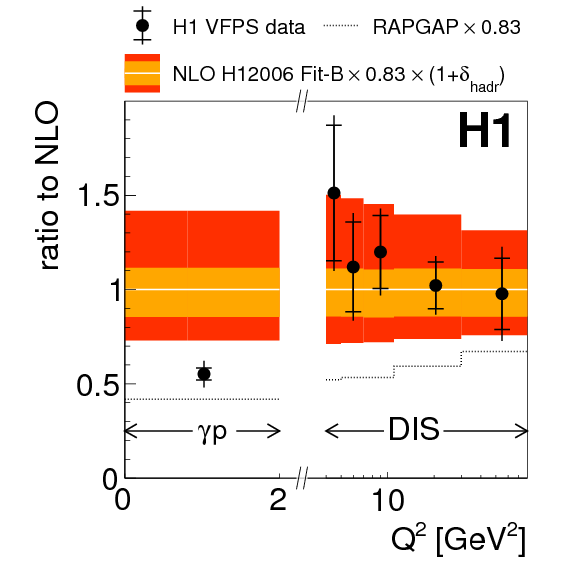
\includegraphics[width=3in]{Chapter1/importfigs/fig8_h1_2015.png}
\par\end{centering}
\caption{Ratio of H1 data cross-section to NLO-QCD cross-section. \label{fig:h1Ratio}}
\end{figure}

H1 used the Very Forward Proton Spectrometer (VFPS) to trigger on low $Q^2$ protons. The VFPS consists of two Roman Pots located 218 m and 222 m from the H1 interaction-point in the forward direction. The VFPS can detect protons scattered at very low transverse momentum, corresponding to $0.008 < x_{P} < 0.028$ and $|t|<0.6$. Each of the Roman Pots contains layers of scintillating fibers, which are covered by a layer of scintillator tiles. The fibers readout to photomultipliers, and the tiles both shield from radiation and trigger on protons. The track effiency of VFPS is a remarkable $96 \%$, and the background contamination is kept at $1 \%$ , making the detector excellent for studying diffractive events. Figure \ref{fig:h1BeamEnv} shows the $|t|$ coverage of the Forward Proton Spectrometer (FPS) and VFPS.

\begin{figure}[h!]
\begin{centering}
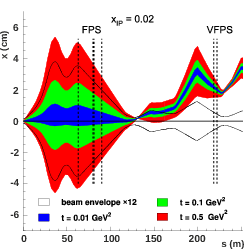
\includegraphics[width=3in]{Chapter1/importfigs/fig7_h1_2015.png}
\par\end{centering}
\caption{Beam envelope vs. distance to vertex in H1. \label{fig:h1BeamEnv}}
\end{figure}

The H1 data was compared to predictions based on NLO-QCD convoluted with diffractive parton distribution functions (DPDFs) from HERA inclusive diffractive deep-inelastic scattering (DDIS) data. For diffractive pp collisions the high transverse momentum jets yield a hard scale for perturbative QCD. 

\subsection{Wigner Distribution}

One can use the Wigner distribution to tomographically image the internal structure of the nucleus \cite{Hatta:2016dxp}. The nucleus manifests different structures at varying momentum fractions; specifically, small momentum fractions exhibit gluon saturation \cite{Boer:2011fh}; see figure \ref{fig:nuclImag} for an illustration of how the nucleus appears at varying momentum fractions.

\begin{figure}[h!]
\begin{centering}
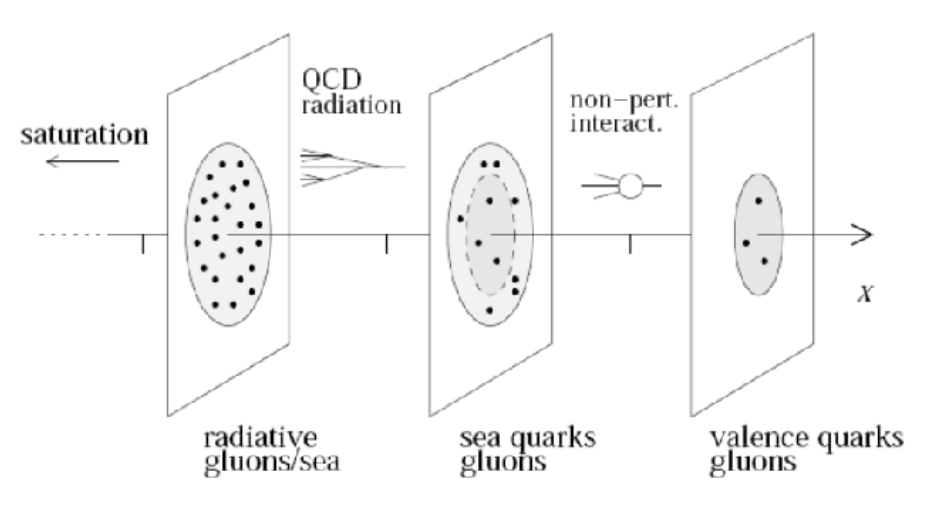
\includegraphics[width=7in]{Chapter1/importfigs/imaging_the_nucleon_upc_dijets_pres.png}
\par\end{centering}
\caption{Subnuclear tomography \label{fig:nuclImag}}
\end{figure}

The quantum field theory lagrangian of the strong interaction is relatively simple, but because of confinement and asymptotic freedom the hadronic bound states are too complex for an analytic solution. Furthermore, collider experiment data requires a quantitative interpretation to be useful. The gap between QCD and heavy-ion data is bridged using the parton model, which considers hadrons as composed of quarks and gluons. Parton density functions (PDFs) model the longitudinal momentum distribution of the partons. PDFs are supplemented by transverse momentum distributions (TMDs) and generalized parton distributions (GPDs). In addition to transverse momentum, GPDs describe the transverse spatial distribution. TMDs and GPDs are derived from the final state particles of a collision. Markus Diehl maps the relationship between various distribution functions in figure \ref{fig:gpdTMDWeb} \cite{Diehl:2003ny}.

The Wigner distribution is a quantum phase space distribution that describes elliptic gluons \cite{Belitsky:2003nz}. Specifically, by considering the color diple scattering amplitude, the angular correlation of the nucleon recoil momentum and the dijet transverse momentum can provide a three-dimensional, tomographic image of the gluons within a high energy nucleus. This tomographic image takes the form of a Wigner distribution, which contains all the information of both TMDs and GPDs without violating the uncertainty principle. Specifically, the angular correlation directly measures the Fourier transform of the gluons. This is possible because the dipole amplitudes are functions of the impact parameter, and because collinear factorization holds. 

\begin{figure}[h!]
\begin{centering}
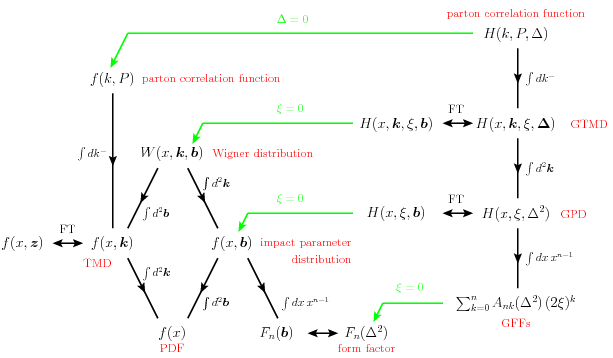
\includegraphics[width=7in]{Chapter1/importfigs/fig6_introGPD_TMD.png}
\par\end{centering}
\caption{Interconnectedness of Parton Distributions. \label{fig:gpdTMDWeb}}
\end{figure}

TMDs and GPDs manifest non-perturbative QCD effects. The Wigner distribution, at this scale, reflects the relationship between the position and momentum of partons. Integrating the Wigner function over the transverse distance yields the TMD, while integrating over transverse momentum yields a GPD with spatial information. 

Yoshitaka Hatta uses the dipole framework to show that the azimuthal angular correlations of coherent dijets are generated by the underlying gluon Wigner distribution. Furthermore, these correlations are consistent with predictions based on standard collinear factorization. Relevant kinematic variables are mapped in the figure \ref{fig:yatta1}.

\begin{figure}[h!]
\begin{centering}
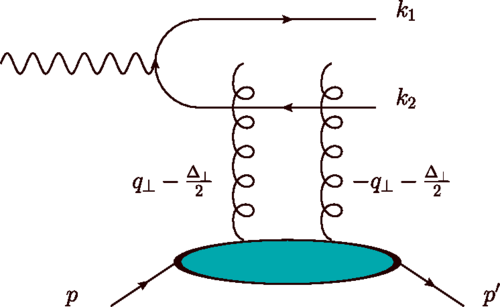
\includegraphics[width=4in]{Chapter1/importfigs/fig4_yatta.png}
\par\end{centering}
\caption{Feynman Diagram of Coherent Dijets in Dipole Framework. \label{fig:yatta1}}.
\end{figure}

It is expected that the dominant contribution to the angular correlation is the ellipitic, corresponding to $n=1$ in the Fourier transform. The interior of the proton displays an intricate structure. 